%% 内容梗概

%% プリアンブル %%%%%%%%%%%%%%%%%%%%%%%%%%%%%%%%%%%%%%%%%%%%%%%%%%%%%%%%
\documentclass[a4j]{jarticle}

\usepackage{kut-abstract}
\usepackage[dvipdfmx]{graphicx}


%% 表題 %%%%%%%%%%%%%%%%%%%%%%%%%%%%%%%%%%%%%%%%%%%%%%%%%%%%%%%%%%%%%%%%
\ScInfo         %% 情報学群生以外の場合はコメントアウトする

\Bachelor	%% 学士学位論文(卒業研究)梗概の場合

\years{平成26}
\title{WebRTC を利用したブラウザキャッシュ共有によるデータ配信システム}
\idnumber{1150361}
\author{松下 和生}
\affiliate{植田研究室}

%% 本文 %%%%%%%%%%%%%%%%%%%%%%%%%%%%%%%%%%%%%%%%%%%%%%%%%%%%%%%%%%%%%%%%
\begin{document}
\begin{Abstract}

  \section{はじめに}
  近年、インターネット上の動画配信によるネットワークトラフィックの急増、
  それによるサーバーへの負荷集中が問題となっている。
  これらの通信の大部分は、HTTP プロトコルを代表とした、 クライアント・サーバー型通信が担っており、
  この通信モデルが通信トラフィックの増加、サーバーへの負荷集中の原因である。
  %
  この問題を解決する既存技術として、P2P Web Proxy が存在するが、いくつか後述の問題が存在する。

  そこで本稿では、この問題を解決したデータ配信システムを設計・提案するとともに、 
  実際にウェブブラウザのプラグインとして実装した結果を報告する。
  
%% ---------------------------------------------------------------------
  
  \section{P2P Web Proxy}
  P2P Web Proxy は、Web Proxy 技術を利用したデータ配信システムであり、
  ウェブサーバーからデータをダウンロードする際、
  P2P Web Proxy を起動している他のピアからのダウロードも並行して行う。

  ピアが LAN などの限られたネットワーク内に存在する場合、
  通信は内部で完結し、インターネット上を流れることがない。
  よって、インターネット上の通信トラフィックが削減され、
  サーバーの負荷軽減に繋がる。

  しかし、P2P Web Proxy には3つの既存の問題が存在する。
  ファイルのダウンロード後もキャッシュを保持しなければいけない問題、
  ウェブブラウザと別にソフトウェアを起動しなければいけない問題、
  外部に向けてポートを開放しておかなければいけない問題である。
  
  この問題を解決したシステムを提案、実装する。
  
%% ---------------------------------------------------------------------
  
  \section{WebRTC を利用したブラウザキャッシュ共有システム}
  ウェブブラウザのプラグインを用いたデータ配信システムを提案する。
  これは、P2P Web Proxy をブラウザのプラグインとして実装したものであり、
  ウェブサーバとの通信に、従来の HTTP プロトコルを用いた方法と、
  WebRTC を用いて他のピアからデータを受信する方法を併用することができる (図 \ref{fig:all})。
  
  \begin{figure}[!t]
    \centering
    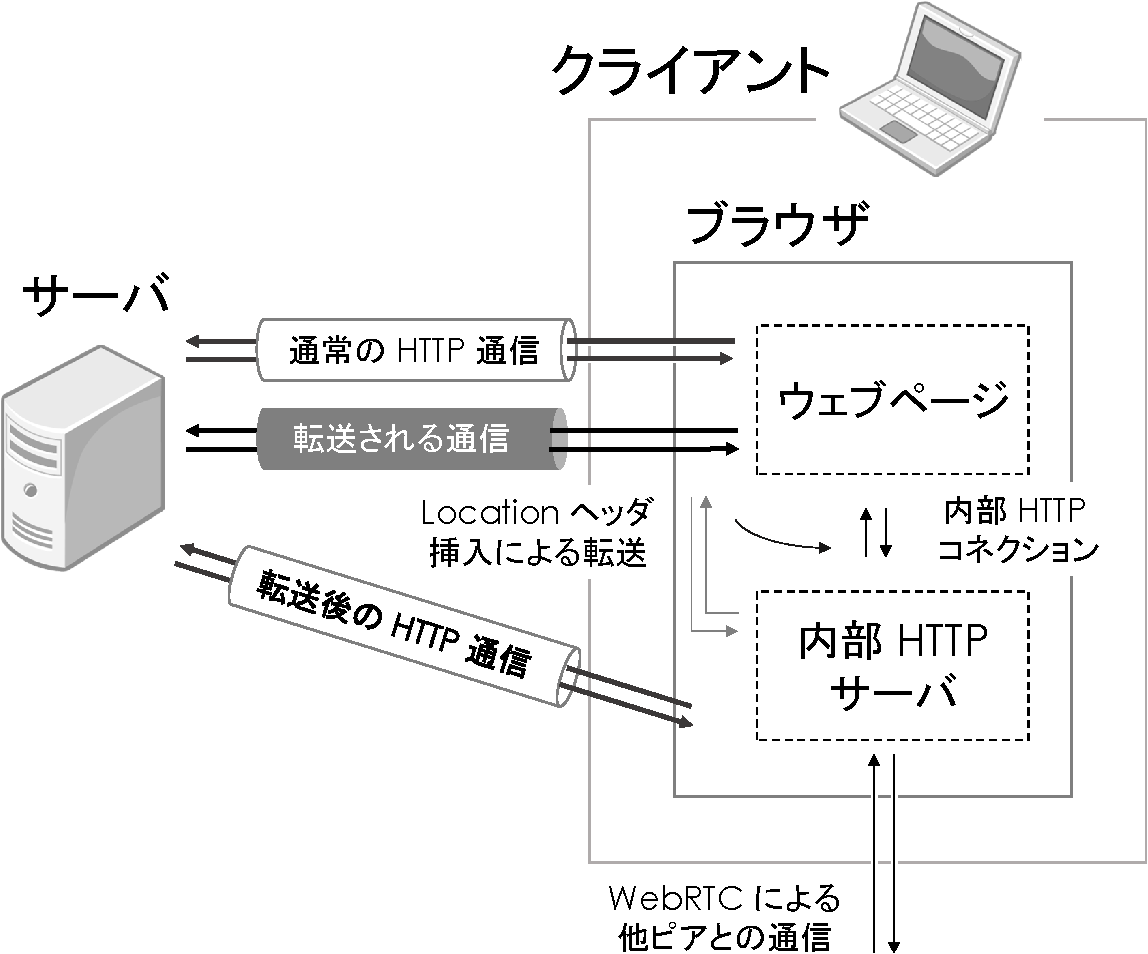
\includegraphics[width=5in]{figure/all.pdf}
    \caption{ブラウザキャッシュ共有システムの概念図}
    \label{fig:all}
  \end{figure}
  
  本システムに対応したウェブサーバーは、
  HTTP ヘッダを用いて対応している旨をクライアントに通知する。
  クライアントは、そのヘッダを検出し、本システムを利用したダウンロードに切り替える。
  そのため、従来の HTTP 通信と併用でき、既存のシステムに対して容易に組み込むことが可能である。
  
  ダウンロードしたデータは通信が終了した時点で破棄される。
  これにより、クライアントがキャッシュを保持し続ける問題を解消している。
  %
  他ピアとの通信には WebRTC を用いる。
  これにより、ポート開放などの作業が不要となり、導入が容易になった \cite{bib:webrtc}。
  
  \section{WebRTC を利用したブラウザキャッシュ共有システムの実装}
  提案システムを、ウェブブラウザである Google Chrome 上で動作するプラグインとして実装した (図 \ref{fig:impl})。
  実装したプラグインは、OS 及び CPU に非依存な技術で構築されているため、
  追加のソフトウェアを要求せず、多くのクライアントで動作させることができる。
  
  \begin{figure}[!t]
    \centering
    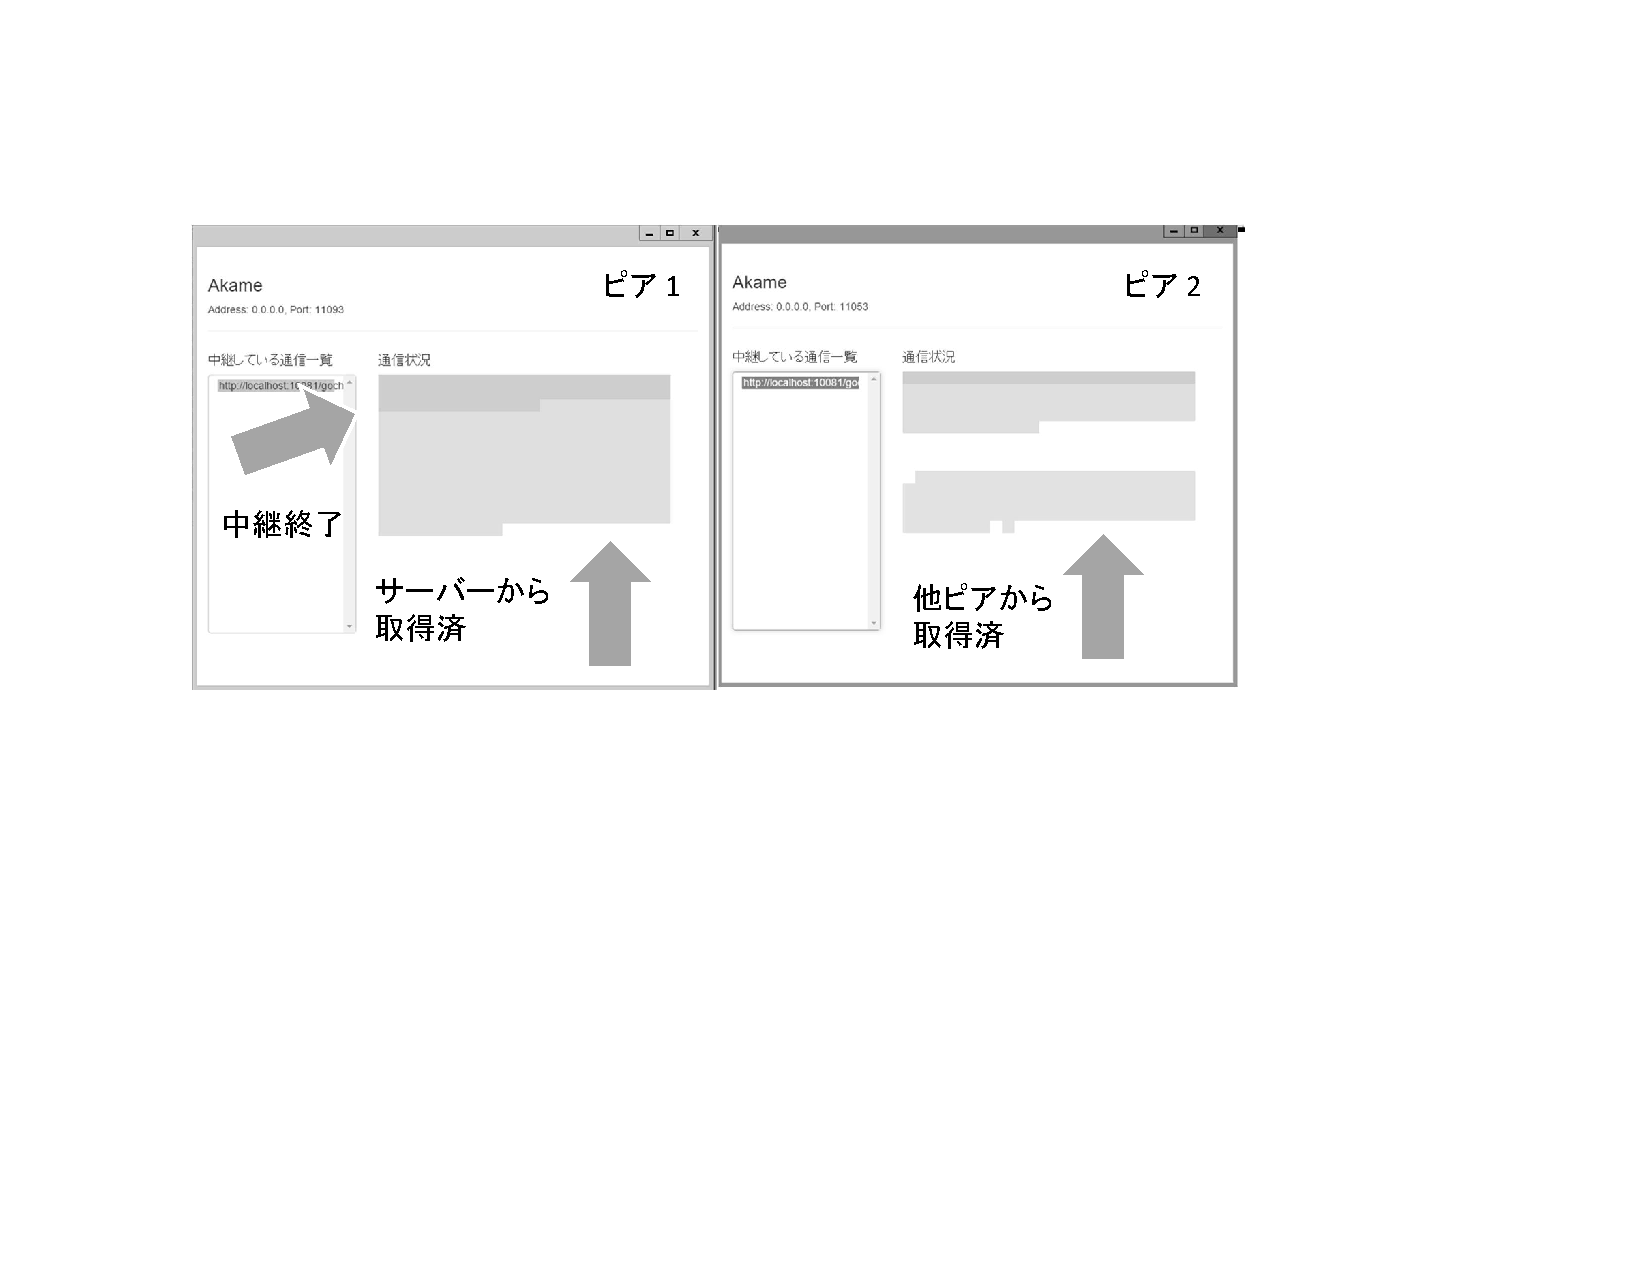
\includegraphics[width=3in]{figure/app.pdf}
    \caption{ブラウザキャッシュ共有システム稼働時の様子}
    \label{fig:impl}
  \end{figure}
  
  \section{まとめ}
  本稿で提案するシステムを用いることにより、通信トラフィックの削減、
  およびウェブサーバ負荷の削減が行えた。
  クライアントへの導入も、既存技術よりも容易に行えた。

%% 参考文献 %%%%%%%%%%%%%%%%%%%%%%%%%%%%%%%%%%%%%%%%%%%%%%%%%%%%%%%%%%%%
\begin{thebibliography}{99}
  \bibitem{bib:webrtc} Alan B. Johnston, Daniel C. Burnett, 内田直樹, 
    ``WebRTC ブラウザベースのP2P技術'',
    リックテレコム,2014.
\end{thebibliography}

\end{Abstract}
\end{document}
